% !TeX root = _main.tex
% ROLE 3 -- TO-BE, DANH GIA, KICH BAN CHIEN LUOC, TRAI NGHIEM KHACH HANG, KET LUAN (muc 8--11).
% Nguoi nhan: nhom tu dien. Muc tieu: 6--8 trang noi dung chinh.
% DUOC SUA: file nay, figures/r3_*; nhan \label bat dau bang r3:.
% KHONG SUA: role_1.tex, role_2.tex, cac file dieu phoi; thong nhat voi role 2
% truoc khi thay du lieu analysis/. Khong sua tay bang sinh tu Python.
% DAU VAO: tables/tab_{comparison,shift_plan,sensitivity,risk}.tex, tables/tab_ext_*.tex.

\section{Phương án cải tiến và phân bổ nhân lực}
\label{r3:tobe}
\subsection{Ba phương án đối chứng}
\begin{table}[htbp]\centering\small
\caption{Thiết kế các phương án trong so sánh mô phỏng}\label{r3:scenarios-design}
\begin{tabularx}{\linewidth}{@{}p{26mm}Y Y Y@{}}
\toprule
Thành phần & A0: AS-IS & A1: lịch theo giờ & A2: số hóa + lịch \\
\midrule
Số kênh $c_t$ & 6 cả ngày & Tối ưu BT1 với $E[S]$ hiện tại & Tối ưu BT1 với $E[S]$ TO-BE \\
$E[S]$ (phút/xe) & xe máy 1,5; ô tô 4,0 & như A0 & giảm 20\%: 1,2; 3,2 \\
Thanh toán & Tiền mặt/QR tại trụ & như A0 & Trả trước QR/ứng dụng, chọn sẵn số tiền \\
Giờ nhân viên/ngày & 96 & 88 & 72 \\
Mục đích & Mốc hiện trạng & Tác động riêng của lịch & Tác động kết hợp lịch + số hóa \\
\bottomrule
\end{tabularx}
\end{table}
So sánh A0--A1 tách được tác động của việc xếp lịch theo giờ; so sánh A1--A2
tách được tác động của số hóa thanh toán (với lịch được tối ưu lại tương ứng).

\subsection{Bài toán lập lịch theo giờ (BT1)}
Với $k=58\,000$ đồng/giờ nhân viên và 16 khung một giờ:
\begin{align}
\min_{c_1,\ldots,c_{16}}\quad & k\textstyle\sum_{t=1}^{16}c_t \\
\text{với}\quad & c_t\in\{1,\ldots,8\},\ \rho_t<1,\ E[W_{q,t}]\le2\text{ phút},\ P(W_{q,t}>5)\le0{,}05. \nonumber
\end{align}
Chi phí cộng theo giờ và ràng buộc tách theo giờ, nên chọn $c_t$ nhỏ nhất khả thi
cho từng giờ là tối ưu trong mô hình. Đây là kế hoạch công suất; lịch ca cá
nhân (ca 4--8 giờ, nghỉ giữa ca) cần thêm một bước ghép ca.
\resulttable{tab_shift_plan.tex}{Số kênh theo giờ của ba phương án}{r3:staffing}
\begin{figure}[htbp]\centering
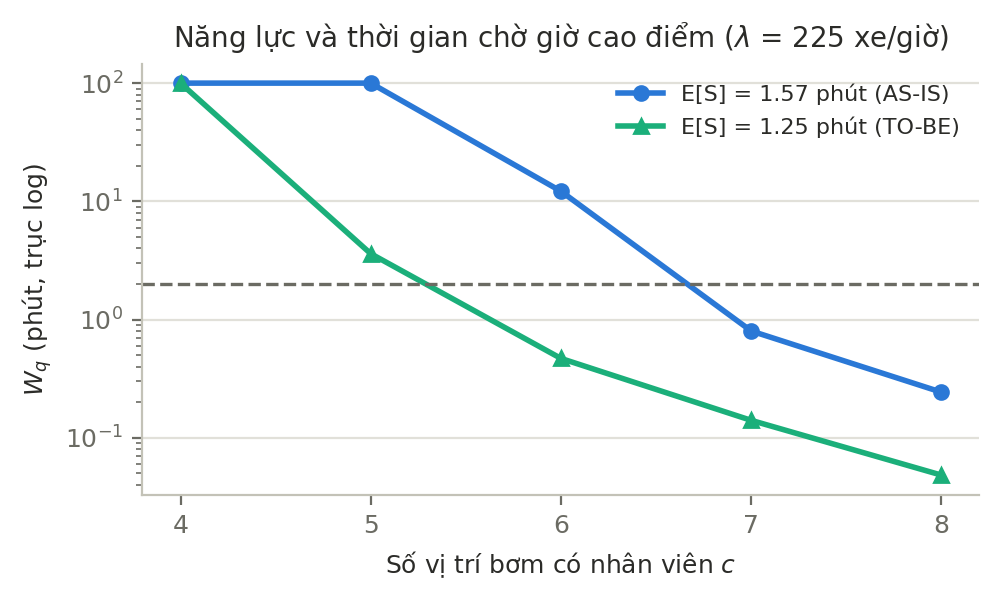
\includegraphics[width=0.82\linewidth]{figures/fig_wq_vs_c.png}
\caption{Thời gian chờ giờ cao điểm theo số kênh (M/M/c).}\label{r3:wq-c}
\source{\texttt{analysis/run\_analysis.py}; tham số Bảng~\ref{r2:assumptions}}
\end{figure}
A1 dồn nhân viên vào 07--09 và 16--19 (6--7 kênh) và rút về 4--5 kênh lúc vắng;
tổng giảm từ 96 xuống 88 giờ/ngày nhưng giờ cao điểm lại nhiều kênh hơn A0.
A2 cần 72 giờ/ngày vì mỗi kênh phục vụ được 47,8 thay vì 38,3 xe/giờ.

\subsection{Quy trình TO-BE}
\begin{figure}[htbp]\centering
\resizebox{\linewidth}{!}{%
\begin{tikzpicture}
\def\W{18.4}
\foreach \y/\name in {0/Khách hàng,-2.4/Nhân viên bơm,-4.8/Ứng dụng / POS / HĐĐT}{
  \draw (0,\y) rectangle (\W,\y-2.4);
  \draw (0.8,\y) -- (0.8,\y-2.4);
  \node[rotate=90,font=\scriptsize\bfseries] at (0.4,\y-1.2) {\name};}
\node[ev] (st) at (1.6,-1.2) {};
\node[task] (t0) at (3.4,-1.2) {Chọn số tiền,\\trả trước QR};
\node[task] (s0) at (3.4,-6.0) {Tạo mã đơn,\\hiển thị ETA};
\node[gw] (g1) at (6.0,-1.2) {Hàng chờ\\$\ge$ 20 xe?};
\node[evend] (eb) at (7.7,-0.45) {};
\node[font=\scriptsize,anchor=west] at (8.1,-0.45) {bỏ đi};
\node[task] (t2) at (8.8,-1.6) {Xếp hàng\\chờ tới lượt};
\node[task] (t3) at (11.2,-3.6) {Quét mã,\\bơm đúng số tiền};
\node[task] (s1) at (13.6,-6.0) {HĐĐT tự động\\gửi về ứng dụng};
\node[task] (t7) at (15.8,-1.2) {Rời trụ\\(không thu tiền)};
\node[evend] (en) at (17.7,-1.2) {};
\node[task,dashed] (pl) at (8.8,-6.0) {Lịch $c_t$ theo\\dự báo (BT1 + GLM)};
\draw[flow] (st) -- (t0);
\draw[msg] (t0) -- (s0);
\draw[flow] (t0) -- (g1);
\draw[flow] (g1.north) |- node[pos=0.25,left,font=\scriptsize]{có} (eb);
\draw[flow] (g1.east) -- node[above,font=\scriptsize]{không} ++(0.6,0) |- (t2);
\draw[flow] (t2) |- (t3);
\draw[flow] (t3) -| (s1);
\draw[flow] (s1) -| (t7);
\draw[flow] (t7) -- (en);
\draw[msg] (pl) -| (t3);
\node[tmark] at (11.2,-4.35) {$S$ giảm 20\%: không thu tiền mặt};
\end{tikzpicture}}
\caption{Quy trình TO-BE: thanh toán trước khi vào trụ, hóa đơn tự động, số nhân viên theo dự báo. Khách không dùng ứng dụng vẫn đi theo luồng AS-IS ở Hình~\ref{r1:bpmn}.}
\label{r3:bpmn}
\source{nhóm vẽ bằng TikZ theo ký pháp BPMN rút gọn; Claude Code hỗ trợ dựng mã hình}
\end{figure}
Thay đổi chính là đưa thanh toán và xuất hóa đơn ra khỏi thời gian chiếm trụ.
Kênh tiền mặt vẫn giữ cho khách lớn tuổi (Mục~\ref{r3:cx}); nếu tỷ lệ khách
dùng trả trước thấp, mức giảm $E[S]$ sẽ nhỏ hơn 20\% (rủi ro ở Bảng~\ref{r3:risks}).
\FloatBarrier

\section{Đánh giá, độ nhạy và giới hạn}
\label{r3:evaluation}
\subsection{So sánh trên cùng bộ chỉ số}
\resulttable{tab_comparison.tex}{Kết quả mô phỏng chính: 20 ngày, cùng seed, CV = 0,8}{r3:comparison}
\begin{itemize}
\item \textbf{Lịch theo giờ (A1) giải quyết phần lớn vấn đề mà không cần đầu tư.}
Trong giờ 17--19, tỷ lệ chờ quá 5 phút giảm từ 6,18\% xuống 0,50\%, tỷ lệ bỏ đi
từ 2,26\% xuống 0,17\%, đồng thời giảm 8 giờ nhân viên/ngày (464 nghìn đồng/ngày).
\item \textbf{Số hóa (A2) chủ yếu tiết kiệm nhân lực.} Thời gian chờ chỉ giảm
thêm ít (0,45 $\rightarrow$ 0,43 phút cả ngày; 0,56 $\rightarrow$ 0,36 phút giờ
17--19), nhưng giảm thêm 16 giờ/ngày. Sau khi trừ 250 nghìn đồng/ngày chi phí số
hóa, A2 rẻ hơn A1 678 nghìn đồng/ngày và rẻ hơn A0 1,14 triệu đồng/ngày
(khoảng 34 triệu đồng/tháng).
\item Ô tô và xe máy dùng chung hàng nên thời gian chờ gần như nhau (A0: 0,59
và 0,64 phút); ô tô chỉ làm tăng $E[S]$ bình quân.
\end{itemize}
\begin{figure}[htbp]\centering
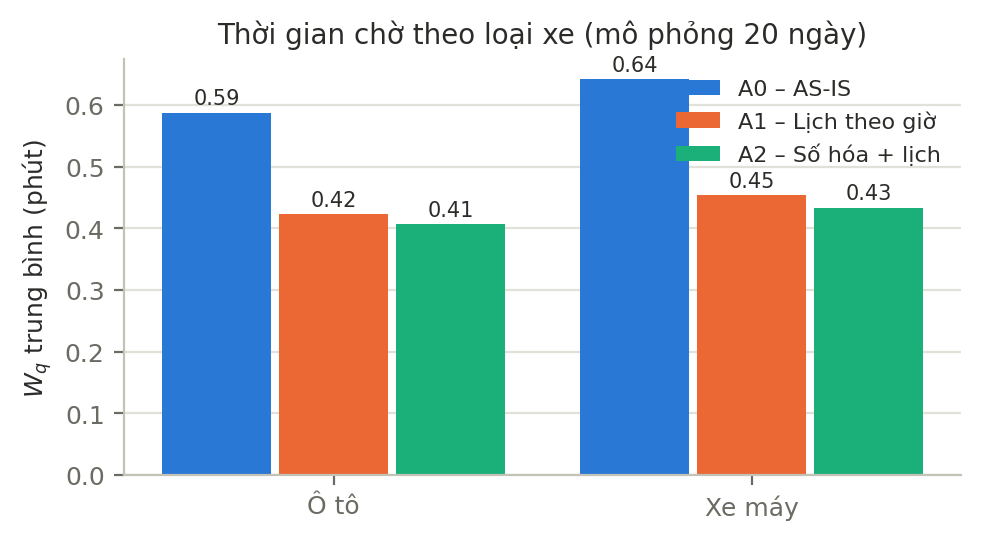
\includegraphics[width=0.82\linewidth]{figures/fig_by_class.png}
\caption{Thời gian chờ theo loại xe của ba phương án.}\label{r3:by-class}
\source{\texttt{analysis/run\_analysis.py}; dữ liệu mô phỏng}
\end{figure}
\FloatBarrier

\subsection{Độ nhạy theo nhu cầu}
\resulttable{tab_sensitivity.tex}{Độ nhạy theo hệ số nhu cầu (30 ngày, seed riêng, giữ nguyên lịch)}{r3:sensitivity}
\begin{figure}[htbp]\centering
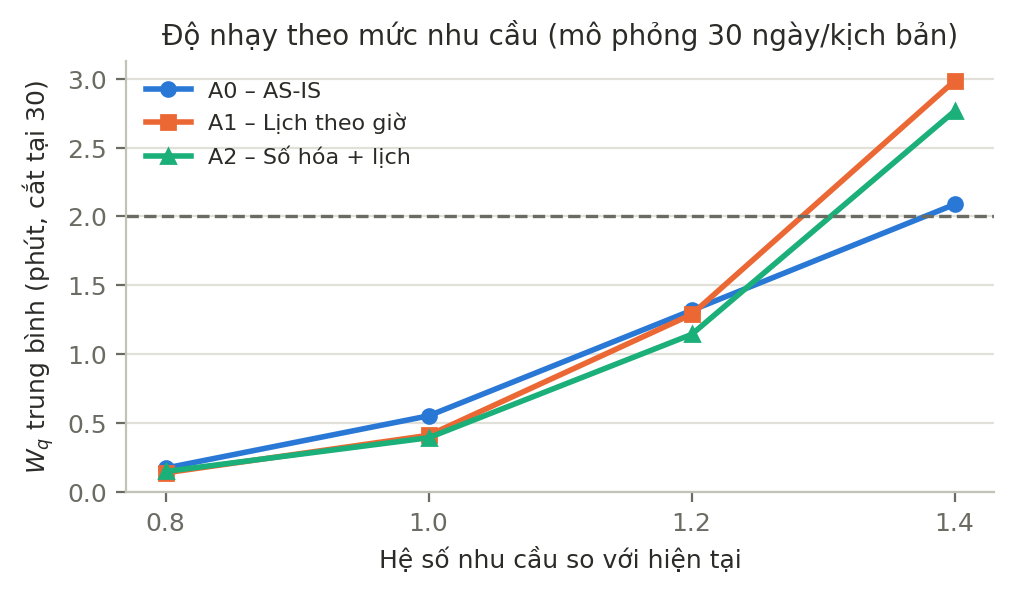
\includegraphics[width=0.85\linewidth]{figures/fig_sensitivity.png}
\caption{Thời gian chờ trung bình khi nhu cầu thay đổi, giữ nguyên lịch.}\label{r3:sens-fig}
\source{\texttt{analysis/run\_analysis.py}; 30 ngày mô phỏng mỗi cấu hình}
\end{figure}
Khi nhu cầu tăng 20\%, cả ba lịch \emph{giữ nguyên} đều có $\rho$ giờ cao điểm
gần hoặc vượt 1; A2 vẫn đạt $P(W_q{>}5)=2{,}61\%$ nhưng 0,53\% khách bỏ đi.
Khi tăng 40\%, mọi lịch đều hỏng (4,9--7,9\% khách bỏ đi). Một lịch tĩnh, dù
tối ưu cho tải cơ sở, không bền trước biến động nhu cầu --- đây là lý do của
BT3 và BT4 ở Mục~\ref{r3:scenarios}.

\subsection{Rủi ro và giới hạn}
\resulttable{tab_risk.tex}{Các tình huống rủi ro của A2 (30 ngày, seed riêng)}{r3:risks}
Thiếu một nhân viên ở mọi giờ làm $P(W_q{>}5)$ tăng lên 16,80\% và 1,93\% khách
bỏ đi: A2 tiết kiệm nhân lực nên ít dư địa. Nếu số hóa chỉ giảm 10\% thời gian
phục vụ, A2 vẫn đạt mục tiêu (1,45\%; 0,10\% bỏ đi). Các giới hạn cần giữ:
\begin{itemize}
\item Lượt xe theo giờ và thời gian phục vụ là mô phỏng; quy mô được hiệu chỉnh
từ số liệu công bố nhưng chưa đo tại một cửa hàng cụ thể.
\item Mô hình coi mọi vòi phục vụ mọi loại xe; thực tế có trụ riêng cho ô tô.
\item Ngưỡng bỏ đi 20 xe và các tham số trải nghiệm khách hàng là giả định.
\item Mỗi ngày bắt đầu với hàng rỗng; kiểm chứng ở tải rất cao còn lệch (Mục~\ref{r2:diagnosis}).
\end{itemize}

\section{Kịch bản chiến lược và trải nghiệm khách hàng}
\label{r3:scenarios}
\subsection{Ba kịch bản tương lai và hai lựa chọn chiến lược}
Từ PESTEL (Bảng~\ref{r1:pestel}), nhóm xây ba kịch bản cho cửa hàng ở tầm
12--24 tháng. Xác suất chỉ dùng để tính chi phí kỳ vọng; tiêu chí chính là
hối tiếc tối đa, không phụ thuộc xác suất.
\begin{itemize}
\item \textbf{KB-A -- Nhu cầu thấp} (0,30): lượt xe $\times0{,}8$ do vùng phát
thải thấp mở rộng và khách chuyển sang xe điện~\cite{ct20,lez2026}.
\item \textbf{KB-B -- Nhu cầu tăng} (0,45): lượt xe $\times1{,}2$ do cửa hàng lân
cận đóng cửa vì chiết khấu thấp~\cite{chietkhau} và xe máy mới tăng~\cite{reg2025}.
\item \textbf{KB-C -- Gián đoạn} (0,25): như đợt tháng 3/2026~\cite{vtc2026},
khách dồn sang ($\times1{,}35$) và bán có kiểm soát làm thời gian phục vụ tăng 15\%.
\end{itemize}
Lựa chọn \textbf{CL-A -- nhân lực theo lịch, không số hóa} giữ lịch A1 (88 giờ).
Lựa chọn \textbf{CL-B -- số hóa} có hai biến thể: \emph{tĩnh} giữ lịch A2 (72 giờ);
\emph{thích ứng} dùng dự báo (Mục~\ref{r2:forecast}) để tối ưu lại $c_t$ theo
BT1 mỗi ngày, phần giờ vượt lịch A2 do nhân viên bán thời gian đảm nhận với đơn
giá $1{,}5\times58\,000$ đồng/giờ. Mỗi ô mô phỏng 30 ngày, cùng seed trong một
kịch bản.

\subsection{Mô hình mất khách theo thế hệ}
\label{r3:cx}
Mục tiêu dài hạn của chiến lược là khách quay lại, không bỏ cửa hàng. Một khách
thuộc phân khúc $g$ đã chờ $w$ phút có xác suất không hài lòng đến mức lần sau
bỏ đi là
\begin{equation}
p_g(w)=1-\exp\!\left[-(w/\theta_g)^2\right],
\end{equation}
dạng Weibull để chờ ngắn gần như không gây mất khách còn chờ dài làm xác suất
tăng nhanh; khách bỏ đi vì hàng dài có $p=1$. Mỗi lượt mất gây thiệt hại
$p\times[\text{lãi gộp lượt đó}+c_g\times\text{CLV}]$, với $c_g$ là xác suất
chuyển hẳn sang cửa hàng khác. CLV là lãi gộp 3 năm của một khách quen: xe máy
$73\times2{,}5\times1\,500\times3\approx820$ nghìn đồng, ô tô
$52\times30\times1\,500\times3\approx7{,}02$ triệu đồng. Các giá trị $\theta_g$,
$c_g$ trong Bảng~\ref{r3:segments} là giả định để thể hiện cơ chế, chưa có khảo sát.
\exttable{tab_ext_segments.tex}{Tỷ lệ mất khách theo phân khúc trong KB-B; $\theta_g$, $c_g$ là giả định}{r3:segments}
\textbf{Nhận định.} Với cùng một hàng chờ, Gen Z mất 8,79\% ở A0 so với 4,77\%
ở nhóm 60+. Khi chờ đã ngắn (CL-B thích ứng), khoảng cách tương đối còn lớn
hơn (1,41\% so với 0,50\%, gấp 2,8 lần): nhóm trẻ --- nhiều người là sinh viên
và tài xế giao hàng --- là nhóm đầu tiên rời đi và cũng là nhóm chuyển sang xe
điện sớm nhất. Hàm ý: thông báo thời gian chờ dự kiến và trả trước trên ứng
dụng cho nhóm trẻ; giữ thu tiền mặt và nhân viên hỗ trợ cho nhóm lớn tuổi.

\subsection{Kết quả theo kịch bản}
\exttable{tab_ext_scenarios.tex}{Hiệu quả của các chiến lược trong ba kịch bản; chi phí và giá trị mất tính bằng nghìn đồng/ngày}{r3:scen-table}
\begin{figure}[htbp]\centering
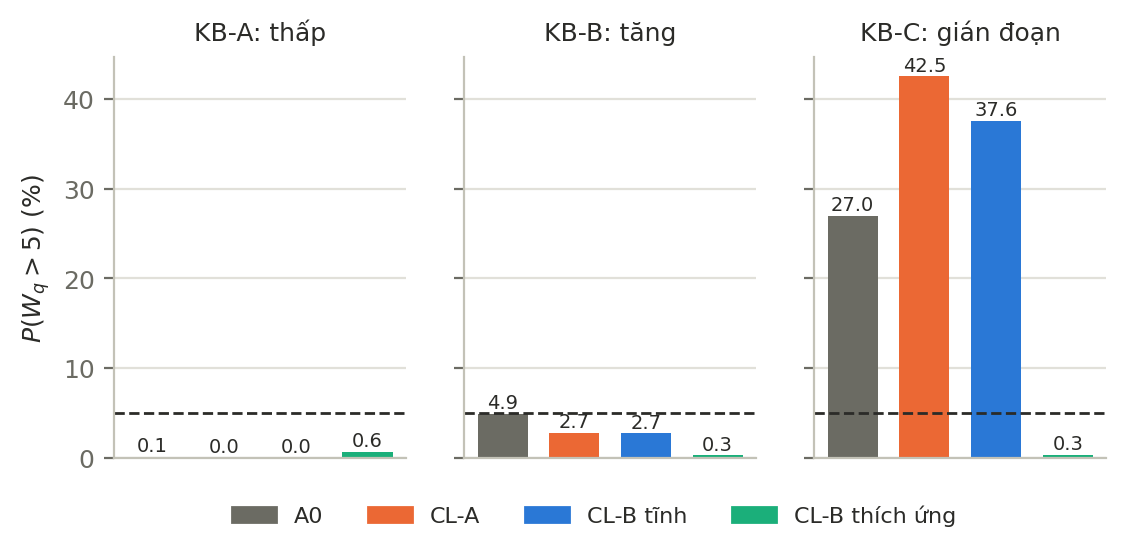
\includegraphics[width=0.92\linewidth]{figures/r3_scenarios.png}
\caption{Tỷ lệ xe chờ quá 5 phút theo kịch bản; đường đứt là mục tiêu 5\%.}
\label{r3:scen-fig}
\source{\texttt{analysis/extension\_analysis.py}; dữ liệu mô phỏng}
\end{figure}
(1) Ở KB-A mọi lựa chọn đều đạt; CL-B tĩnh rẻ nhất (4,68 triệu đồng/ngày) vì
biến thể thích ứng cắt xuống 59 giờ và làm chờ tăng nhẹ. (2) Ở KB-B, lịch tĩnh
vẫn đạt $P(W_q{>}5)\le5\%$ nhưng 3,6--4,4\% khách bị mất; CL-B thích ứng tăng lên
81 giờ và chỉ mất 0,98\%. (3) KB-C quyết định lựa chọn: mọi lịch tĩnh đều sụp
(37,6--42,5\% xe chờ quá 5 phút, 11,8--13,6\% bỏ đi), trong khi CL-B thích ứng
giữ 0,30\% với 101 giờ/ngày --- gần chạm giới hạn 8 vòi ở giờ cao điểm.
\exttable{tab_ext_regret.tex}{Tổng chi phí (nghìn đồng/ngày), kỳ vọng và hối tiếc tối đa; ``đạt'' khi $P(W_q{>}5)\le5\%$ và bỏ đi $\le1\%$}{r3:regret}

\subsection{Đánh giá và quyết định}
Nhóm chọn \textbf{CL-B thích ứng}: hối tiếc tối đa chỉ 554,8 nghìn đồng/ngày
(ở KB-A) so với 59--66 triệu đồng/ngày của hai lựa chọn tĩnh (ở KB-C); chi phí kỳ
vọng 7,31 so với 23,90--26,72 triệu đồng/ngày; và là lựa chọn duy nhất đạt mục
tiêu ở cả ba kịch bản.
\exttable{tab_ext_clv.tex}{Chi phí kỳ vọng (nghìn đồng/ngày) theo hệ số CLV}{r3:clv}
\textbf{Kết luận có bền không?} Ngay cả khi bỏ hoàn toàn giá trị khách quay lại
(CLV = 0, chỉ tính lãi gộp của lượt bị mất), CL-B thích ứng vẫn rẻ nhất
(5,34 so với 5,87 và 6,71 triệu đồng/ngày) vì khách bỏ đi trong KB-C là doanh
thu mất ngay. Điều kiện để kết luận đúng là \emph{dự báo đủ tốt} và \emph{có
nguồn nhân viên bán thời gian huy động được trong ngày}.

\subsection{Năng lực thích ứng nhờ dự báo}
\label{r3:ml-staff}
Mô hình GLM ở Mục~\ref{r2:forecast} được dùng để lập lịch $c_t$ cho từng ngày
kiểm tra; mỗi ngày được mô phỏng với nhu cầu thật của ngày đó.
\exttable{tab_ext_ml_staff.tex}{Lập lịch theo dự báo trên 84 ngày kiểm tra (5/1--29/3/2026); ngày vi phạm: $P(W_q{>}5)>5\%$ hoặc bỏ đi $>1\%$}{r3:ml-staff-table}
Lịch A2 tĩnh vi phạm ở 16,7\% số ngày và 10,67\% xe chờ quá 5 phút trong các
ngày sự kiện. Lịch theo GLM giảm số ngày vi phạm xuống 6,0\% mà chỉ dùng 70,48
giờ/ngày --- ít hơn lịch tĩnh. Phương án ``đệm 20\%'' đạt kết quả tương đương
(7,1\% ngày vi phạm) nhưng tốn 81 giờ/ngày; GLM tiết kiệm 10,5 giờ, tức 610
nghìn đồng/ngày (khoảng 18 triệu đồng/tháng). Lịch theo trung bình 4 tuần còn
kém lịch tĩnh (27,4\% ngày vi phạm) vì phản ứng trễ với sự kiện.

\begin{table}[htbp]\centering\small
\caption{Kế hoạch ứng phó: dấu hiệu sớm, ngưỡng kích hoạt và hành động}\label{r3:playbook}
\begin{tabularx}{\linewidth}{@{}p{14mm}Y Y Y@{}}
\toprule
Kịch bản & Dấu hiệu sớm & Ngưỡng kích hoạt & Hành động \\
\midrule
KB-A & Lượt xe dự báo giảm; vùng phát thải thấp mở rộng & $<2\,000$ lượt/ngày trong 4 tuần & Giảm kênh lúc vắng; đàm phán lắp tủ đổi pin/trạm sạc~\cite{vgx} \\
KB-B & Cửa hàng lân cận đóng cửa; dự báo tăng & $>2\,900$ lượt/ngày hoặc $\rho_{17-19}>0{,}85$ & Tối ưu lại $c_t$ ($\approx$81 giờ/ngày); tuyển thêm nhân viên bán thời gian \\
KB-C & Tin căng thẳng nguồn cung; điều chỉnh giá lớn & Tín hiệu nguồn cung hoặc $|\Delta p|\ge1\,000$ đồng/lít & Mở đủ 8 vòi giờ cao điểm; gọi ca dự phòng; hiển thị ETA, ưu tiên khách trả trước \\
\bottomrule
\end{tabularx}
\end{table}

\begin{table}[htbp]\centering\small
\caption{Học máy trong dịch vụ: tác động, chỉ số chấp nhận và kiểm soát}\label{r3:ml-uses}
\begin{tabularx}{\linewidth}{@{}p{27mm}Y Y Y@{}}
\toprule
Ứng dụng & Tác động lên mô hình & Chỉ số chấp nhận & Kiểm soát \\
\midrule
Dự báo lượt xe (đã thử) & $\hat\lambda_{d,h}\to c_t$ & MAPE $\le10\%$; ngày vi phạm $\le7\%$ & Cửa hàng trưởng duyệt lịch hằng ngày \\
Ước lượng độ kiên nhẫn & $\theta_g$ từ tỷ lệ bỏ đi theo độ dài hàng & Sai số dự báo bỏ đi & Chỉ dùng dữ liệu ẩn danh, gộp \\
Dự báo rời bỏ & Khách quen giảm tần suất & AUC; tỷ lệ giữ chân & Ưu đãi có đồng ý của khách \\
Phát hiện bất thường & Lượt bán đột biến, lỗi cột bơm & Thời gian phát hiện & Kiểm tra thủ công trước khi xử lý \\
\bottomrule
\end{tabularx}
\end{table}

\section{Kết luận và đề xuất định hướng}
\label{r3:conclusion}
Trong bộ giả định đã hiệu chỉnh theo số liệu công bố, vấn đề của cửa hàng đại
diện không phải thiếu nhân viên mà là \emph{nhân viên đặt sai giờ}: lịch cố định
6 người thừa công suất ban ngày nhưng để 6,2\% xe chờ quá 5 phút và 2,3\% xe bỏ
đi giờ tan tầm. Trung bình cả ngày (0,64 phút) che khuất điểm nghẽn này.

\textbf{Đề xuất.} Nhóm đề xuất chiến lược \textbf{``số hóa có lịch thích ứng''
(CL-B thích ứng)}, triển khai ba bước:
\begin{enumerate}
\item \textbf{0--3 tháng -- Đo và xếp lại lịch.} Xuất dấu thời gian từ hóa đơn
điện tử theo giờ, bấm giờ 30--50 lượt mỗi loại xe; áp dụng ngay lịch theo giờ
(A1): giảm 8 giờ/ngày và đưa tỷ lệ bỏ đi giờ 17--19 từ 2,26\% về 0,17\% mà
không cần đầu tư.
\item \textbf{3--6 tháng -- Số hóa thanh toán.} Trả trước QR/ứng dụng và hóa
đơn tự động; khi $E[S]$ giảm 20\%, lịch còn 72 giờ/ngày, tiết kiệm khoảng 34
triệu đồng/tháng so với hiện trạng. Giữ kênh tiền mặt cho khách lớn tuổi.
\item \textbf{6--12 tháng -- Lịch thích ứng và mở rộng.} Dùng GLM dự báo lượt xe
ngày tới (MAPE 7,25\% trong kiểm tra), lập nhóm nhân viên bán thời gian cho
ngày sự kiện; khi mở cửa hàng mới, ưu tiên \textbf{J3 Hà Đông + J4 Hoàng Mai}
(lãi 163,2 triệu đồng/tháng, bền ở 5/6 tình huống độ nhạy) và chuẩn bị mặt
bằng cho đổi pin/sạc nếu KB-A xảy ra.
\end{enumerate}
Theo dõi bốn KPI theo tháng --- $P(W_q{>}5)$ giờ 17--19, tỷ lệ bỏ đi, tỷ lệ mất
khách theo nhóm tuổi, MAPE dự báo --- và xem lại chiến lược khi một ngưỡng ở
Bảng~\ref{r3:playbook} bị vượt. Các kết luận dựa trên mô phỏng; mức giảm $E[S]$,
ngưỡng bỏ đi, độ kiên nhẫn theo thế hệ và chi phí cố định phải được đo lại tại
cửa hàng thật trước khi triển khai.
\todo{3}{Đối chiếu từng con số trong mục này với \path{analysis/data/run_log.txt}
và \path{analysis/data/ext_run_log.txt} sau lần chạy cuối cùng.}
